\documentclass{article}

\usepackage[utf8]{inputenc} % allow utf-8 input
\usepackage[T1]{fontenc}    % use 8-bit T1 fonts
\usepackage{hyperref}       % hyperlinks
\usepackage{url}            % simple URL typesetting
\usepackage{booktabs}       % professional-quality tables
\usepackage{amsfonts}       % blackboard math symbols
\usepackage{nicefrac}       % compact symbols for 1/2, etc.
\usepackage{microtype}      % microtypography
\usepackage{graphicx}
\usepackage{float}
\usepackage{subcaption}
\usepackage{amsmath}

\title{Cases}
\author{VK}
\date{\today}

\title{Project 4: Implementation, Investigation, and Extensions of Neural Style Transfer for Image Blending}

\author{Sagar Agarwal, sa3633\\Jimmy Kuo, jk4227\\ Siddhanth Sabharwal, ss5689}

\begin{document}

\maketitle

\begin{abstract}

\noindent While Convolutional Neural Networks (CNNs) have been shown to be effective for the purposes of content recognition, they are much less proven for the objective of style representation. Here we implement A Neural Algorithm of Artistic Style and test its effectiveness on various content and style images. We have used pretrained networks and GPU acceleration for speed-up purposes. Our results demonstrate the algorithm's effectiveness on a broad range of settings and parameters. Lastly, we propose and explore an extension related to Many-Artist Style Transfer (MAST).

\end{abstract}

\section{Introduction}

Object detection is a well-studied problem. One of the state-of-the art algorithms in the area is the pretrained image classification network, VGG. It is a nineteen layer neural network with convolution, pooling, and fully-connected layers proposed in 2014 in a paper titled Very Deep Convolutional Networks for Large-Scale Image Recognition by Simonyan and Zisserman. [1] Separating content and style representations in an image is an important task in computer graphics. Aside from texture transfer, the stylization of images is not a well-studied problem. In 2016, the paper Image Style Transfer Using Convolutional Neural Networks by Gatys, Ecker and Bethge proposed a novel algorithm called Neural Algorithm of Artistic Style for the task of style transfer from one image to another. [2] The algorithm they proposed relies on VGG as a building block to recognize objects. They modified the VGG network in three ways. First, they normalized the network so the mean activations is always equal to one. Second, they removed the fully connected layers. Third, they modified the network to do average pooling instead of max pooling. Our objective is to implement the Neural Algorithm of Artistic Style, test its performance on a variety of content and image combinations, observe its robustness to hyperparameter tuning, optimize the algorithm for speed, and propose extensions with interesting applications. Our project is divided into three further sections: the methods we used, the results we obtained, and the conclusions we formed.

\section{Methods}

In this section we outline the theory behind the VGG image embeddings, the Neural Algorithm of Artistic Style, and the MAST extension.

\subsection{Visual Geometry Group (VGG)}

The network which the paper is based on is the VGG-19 network. The VGG-19 network is comprised of a collection of convolutional and pooling layers with a few fully-connected layers. However, in the paper, a modified VGG is used instead, where the fully-connected layers are removed. The resulting network is a normalized VGG-19 with 16 convolutional and 5 pooling layers. Network is normalized by scaling the eights so that the mean activation of each convolutional layer over images and positions is equal to one. 
To fix the notation and the mathematics, et $\vec{x}$ be the given input image. For each layer $l$, there are $N_l$ filters, with each filter having a feature map of size $M_l$. $M_l$ is the height times the width of the map. Therefore, we can store all responses in layer $l$ in a matrix $F^l \in \mathbb{R}^{N_l \times M_l}$. Now we denote $F_{ij}^l$ as the activation of the $i^th$ filter at position $j$ in layer $l$. Therefore now we can write the Sum of Squared loss function between 2 feature representations as 
$$
L_{content}(\vec{p}, \vec{x}, l) = \frac{1}{2}\sum_{i,j} \left(F^l_{ij} - P^l_{i,j}\right)^2
$$
where $P^l_{i,j}$ is the original image counter-part of $F^l_{i,j}$. Minimizing the loss function we have 

$$
\frac{\partial L_{content}}{\partial F^l_{i,j}} = 
\begin{cases}
(F^l - P^l)_{i,j} &\text{if $F^l_{ij} > 0$} \\
0 &\text{if $F^l_{ij} < 0$}
\end{cases}
$$
To solve the maximization problem, back-propagation is used. Therefore $\vec{x}$ is modified until it generates the same response in the CNN as the original image $\vec{p}$. 

\subsection{Neural Algorithm of Artistic Style}

\subsection{Many-Artist Style Transfer (MAST)}

An extension of our project was considering how to blend multiple style images together onto one content image. We were motivated to imagine what would a painting look like if collaborated on by artists of different eras. The modification to the previous methodology is in the total loss function. Given $k$ style images and $k$ weights, $s_{1}, s_{2}, ..., s_{k}$ such that $\sum_{t = 1}^{k} s_{t} = 1$, the contribution of each layer $l$ to the loss function is:

$$E_{l} = \frac{1}{4N_{l}^{2}M_{l}^{2}}\sum_{i, j}(G_{ij}^{l} - \sum_{t = 1}^{k} s_{t}*A_{ijt}^{l}).$$

\noindent The style reconstruction error is now:

$$L_{style} = \sum_{l} w_{l} \frac{1}{4N_{l}^{2}M_{l}^{2}} \sum_{i, j}(G_{ij}^{l} - \sum_{t = 1}^{k} s_{t}*A_{ijt}^{l})$$

\noindent Results for $k = 2$ are shown below, but $k$ can by any positive integer. Note that MAST is a completely generalization of the Neural Algorithm of Artistic Style, and when $k = 1$ MAST simplifies to the Neural Algorithm of Artistic Style.

\section{Results}

In this section we show blended images created from our implementation of the Neural Algorithm of Artistic Style. Then for a single set of content and style images we show our implementation's sensitivity towards the number of training iterations, random seeds, $\frac{Content Weight}{Style Weight}$ ratios, and choice of image embedding. Next, we plot the loss functions as a function of the training iteration and compare the timing performance of our implementation over a CPU and GPU. Lastly, we show the results of the MAST algorithm for a variety of relative weight configurations. 

\subsection{Neural Algorithm of Artistic Style Results}

To demonstrate the effectiveness of our implementation of this algorithm, we chose three different content images and two different style images. For our content images we chose pictures of San Francisco, a female, and a cat. For our style images we chose Starry Night by Vincent Van Gogh and The Great Wave by Katsushika Hokusai. We then ran our algorithm on each combination of one content image and one style image. The hyperparameters for this run were $iterations = 8000, \frac{Content Weight}{Style Weight} = 10^{-7}, seed = 1$, and the image embeddings used are from VGG with $19$ layers. The results are below, the order from left to right of the images in each figure is the content image, the style image, and the blended image:

\begin{figure}[H]
    \centering
    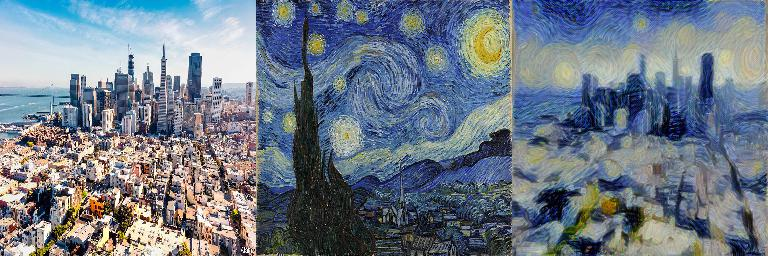
\includegraphics[height=5cm, width=15cm]{sf_van_combined}
    \caption{Content Image: San Francisco, Style Image: Starry Night}
    \label{fig:comb1}
\end{figure}

\begin{figure}[H]
    \centering
    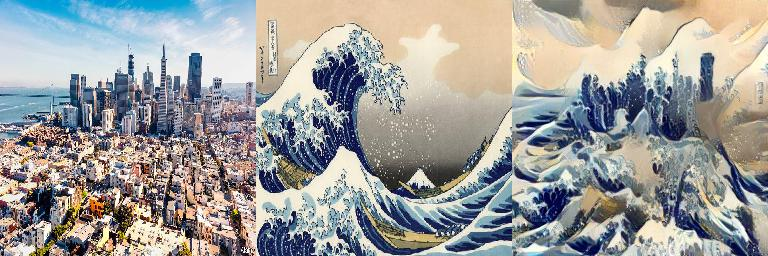
\includegraphics[height=5cm, width=15cm]{sf_wave_combined}
    \caption{Content Image: San Francisco, Style Image: The Great Wave}
    \label{fig:comb2}
\end{figure}

\begin{figure}[H]
    \centering
    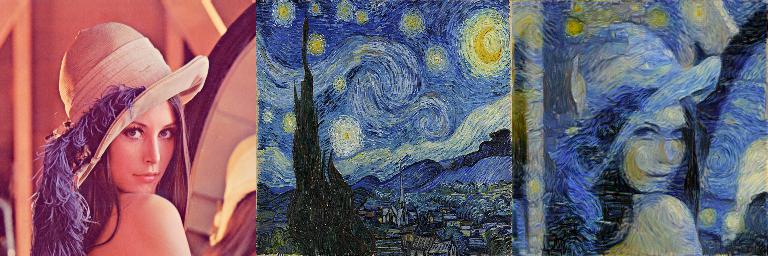
\includegraphics[height=5cm, width=15cm]{female_van_combined}
    \caption{Content Image: Female, Style Image: Starry Night}
    \label{fig:comb3}
\end{figure}

\begin{figure}[H]
    \centering
    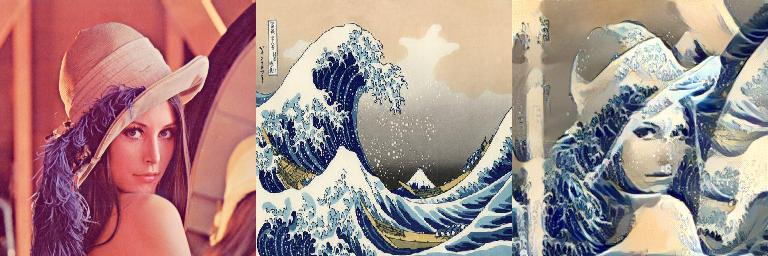
\includegraphics[height=5cm, width=15cm]{female_wave_combined}
    \caption{Content Image: Female, Style Image: The Great Wave}
    \label{fig:comb4}
\end{figure}

\begin{figure}[H]
    \centering
    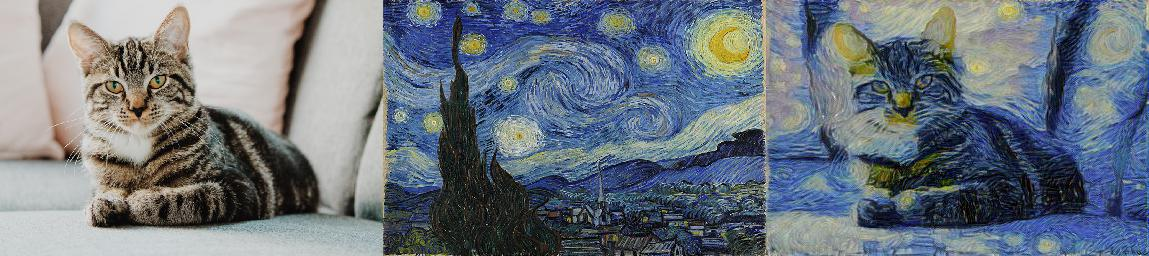
\includegraphics[height=5cm, width=15cm]{cat_van_combined}
    \caption{Content Image: Cat, Style Image: Starry Night}
    \label{fig:comb5}
\end{figure}

\begin{figure}[H]
    \centering
    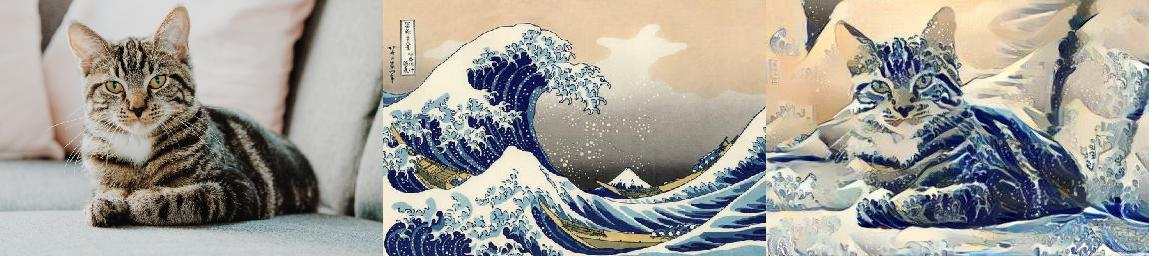
\includegraphics[height=5cm, width=15cm]{cat_wave_combined}
    \caption{Content Image: Cat, Style Image: The Great Wave}
    \label{fig:comb6}
\end{figure}

\noindent We can see that our implementation is effective in extracting style and content embeddings and then blending them together. In general, this shows that the pretrained VGG embedding algorithm is effective.

\subsection{Results over Training Iterations}

We also show what the resulting images look like when the number of training iterations is varied. The hyperparameters for this run were $\frac{Content Weight}{Style Weight} = 10^{-7}, seed = 1$, and the image embeddings used are from VGG with $19$ layers. We chose the cat content image, and the dark style image. The style image is:

\begin{figure}[H]
    \centering
    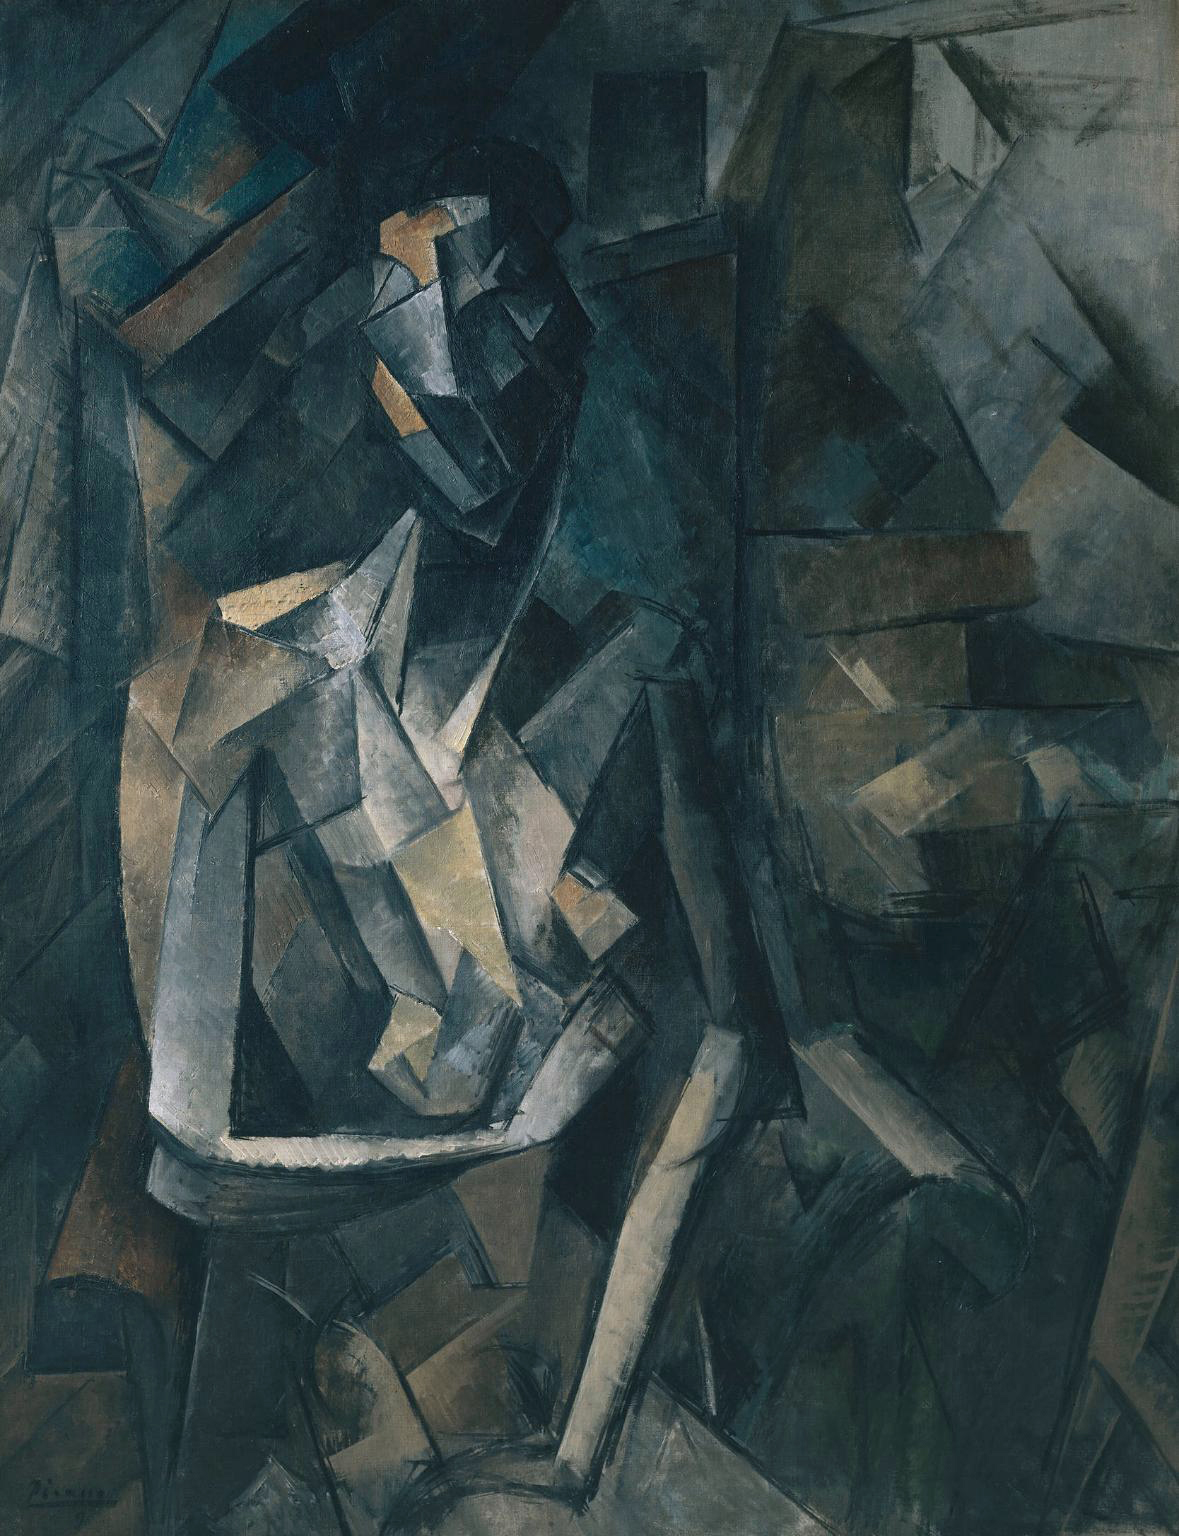
\includegraphics[height=5cm,width=5cm]{dark}
    \caption{Style Image: Dark}
    \label{fig:comb6}
\end{figure}

The results of the blending at various iteration points are below:

\begin{figure}[H]
\begin{subfigure}{.5\textwidth}
  \centering
  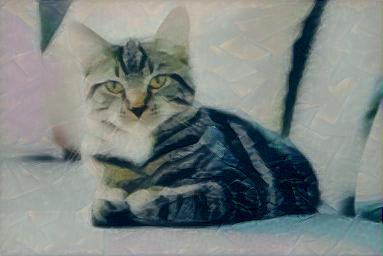
\includegraphics[width=.8\linewidth]{cat_dark_1200}
  \caption{1200 Iterations}
  \label{fig:sfig1}
\end{subfigure}
\begin{subfigure}{.5\textwidth}
  \centering
  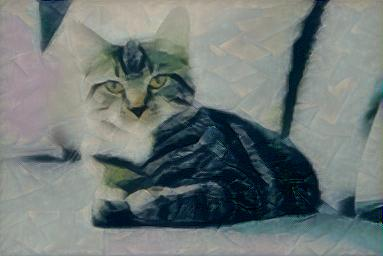
\includegraphics[width=.8\linewidth]{cat_dark_2000}
  \caption{2000 Iterations}
  \label{fig:sfig2}
\end{subfigure}
\begin{subfigure}{.5\textwidth}
  \centering
  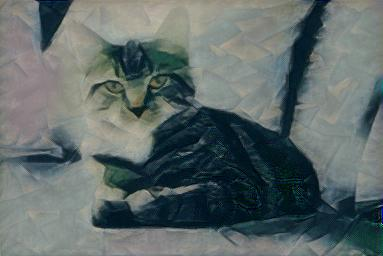
\includegraphics[width=.8\linewidth]{cat_dark_3200}
  \caption{3200 Iterations}
  \label{fig:sfig3}
\end{subfigure}
\begin{subfigure}{.5\textwidth}
  \centering
  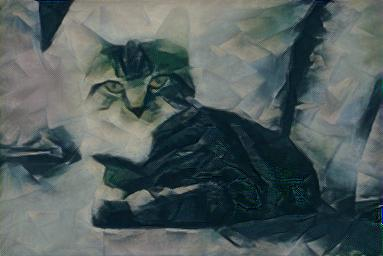
\includegraphics[width=.8\linewidth]{cat_dark_4000}
  \caption{4000 Iterations}
  \label{fig:sfig4}
\end{subfigure}
\begin{subfigure}{.5\textwidth}
  \centering
  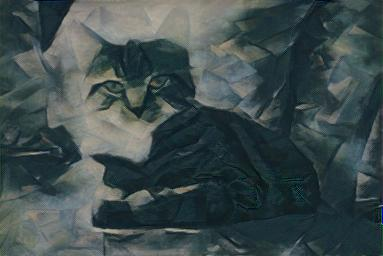
\includegraphics[width=.8\linewidth]{cat_dark_5200}
  \caption{5200 Iterations}
  \label{fig:sfig5}
\end{subfigure}
\begin{subfigure}{.5\textwidth}
  \centering
  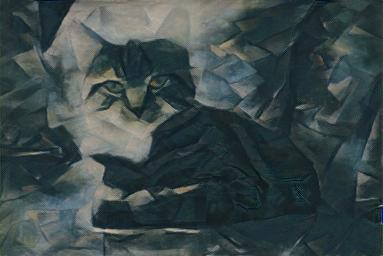
\includegraphics[width=.8\linewidth]{cat_dark_6000}
  \caption{6000 Iterations}
  \label{fig:sfig6}
\end{subfigure}
\begin{subfigure}{.5\textwidth}
  \centering
  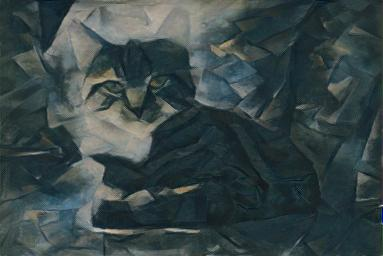
\includegraphics[width=.8\linewidth]{cat_dark_7200}
  \caption{7200 Iterations}
  \label{fig:sfig7}
\end{subfigure}
\begin{subfigure}{.5\textwidth}
  \centering
  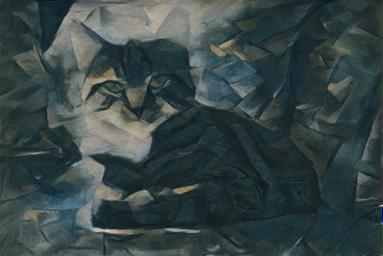
\includegraphics[width=.8\linewidth]{cat_dark_8000}
  \caption{8000 Iterations}
  \label{fig:sfig8}
\end{subfigure}
\caption{Content Image: Cat, Style Image: Dark}
\label{fig:fig}
\end{figure}

\noindent As the iteration count increases we see that the effect of the style image is more pronounced in the target image. This makes sense as the relative weight of the style image is higher than the relative weight of the content image in our base implementation. The results of the blending for various starting seeds are below:

\subsection{Results over Random Seeds}

Since we are running the algorithm in a base configuration with 8000 iterations, we would like to test our implementation over various starting seeds to check its sensitivity. The hyperparameters for this run were $iterations = 8000, \frac{Content Weight}{Style Weight} = 10^{-7}$, and the image embeddings used are from VGG with $19$ layers.

\begin{figure}[H]
\begin{subfigure}{.5\textwidth}
  \centering
  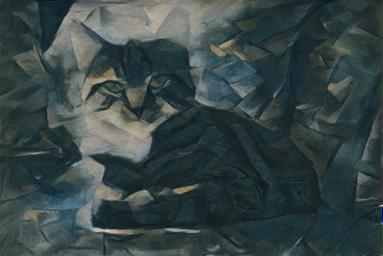
\includegraphics[width=.8\linewidth]{cat_dark_8000}
  \caption{Seed = 1}
  \label{fig:sfig1}
\end{subfigure}
\begin{subfigure}{.5\textwidth}
  \centering
  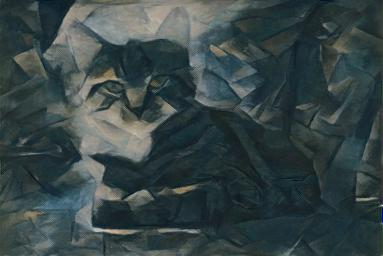
\includegraphics[width=.8\linewidth]{cat_dark2}
  \caption{Seed = 2}
  \label{fig:sfig2}
\end{subfigure}
\begin{subfigure}{.5\textwidth}
  \centering
  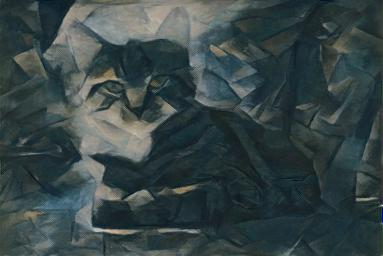
\includegraphics[width=.8\linewidth]{cat_dark3}
  \caption{Seed = 3}
  \label{fig:sfig3}
\end{subfigure}
\begin{subfigure}{.5\textwidth}
  \centering
  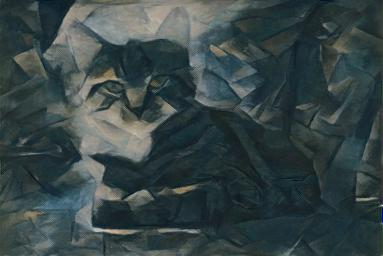
\includegraphics[width=.8\linewidth]{cat_dark4}
  \caption{Seed = 4}
  \label{fig:sfig4}
\end{subfigure}
\caption{Content Image: Cat, Style Image: Dark}
\label{fig:fig}
\end{figure}

\noindent We can see that all the output images are very similar, this means that we are running our algorithm to the point of convergence. It seems that 8000 iterations is a good amount for our implementation.

\subsection{Results over Content Weight:Style Weight Ratios}

Next we want to see what happens to the blended image for different relative weights of the content and style loss in the total loss function. The hyperparameters for this run were $iterations = 8000, seed = 1$, and the image embeddings used are from VGG with $19$ layers. The results are below:

\begin{figure}[H]
\begin{subfigure}{.5\textwidth}
  \centering
  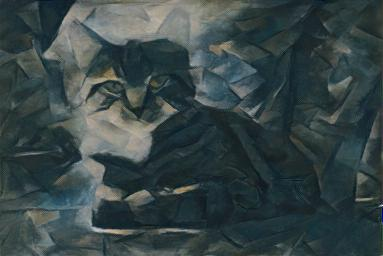
\includegraphics[width=.8\linewidth]{cat_dark1e-07}
  \caption{Ratio = $10^{-8}$}
  \label{fig:sfig1}
\end{subfigure}
\begin{subfigure}{.5\textwidth}
  \centering
  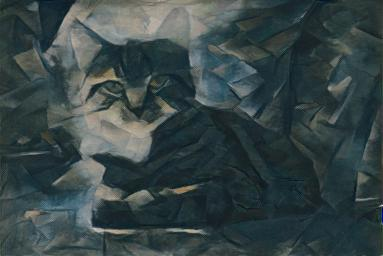
\includegraphics[width=.8\linewidth]{cat_dark1e-05}
  \caption{Ratio = $10^{-6}$}
  \label{fig:sfig2}
\end{subfigure}
\begin{subfigure}{.5\textwidth}
  \centering
  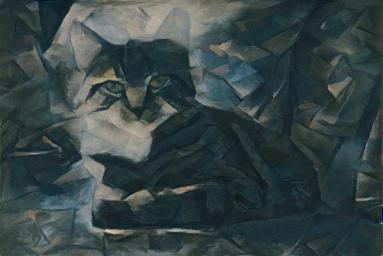
\includegraphics[width=.8\linewidth]{cat_dark1e-04}
  \caption{Ratio = $10^{-5}$}
  \label{fig:sfig3}
\end{subfigure}
\begin{subfigure}{.5\textwidth}
  \centering
  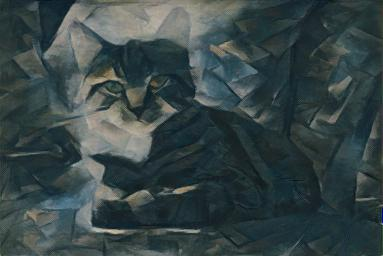
\includegraphics[width=.8\linewidth]{cat_dark1e-03}
  \caption{Ratio = $10^{-4}$}
  \label{fig:sfig4}
\end{subfigure}
\begin{subfigure}{.5\textwidth}
  \centering
  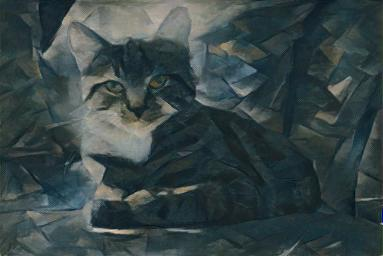
\includegraphics[width=.8\linewidth]{cat_dark1e-02}
  \caption{Ratio = $10^{-3}$}
  \label{fig:sfig5}
\end{subfigure}
\begin{subfigure}{.5\textwidth}
  \centering
  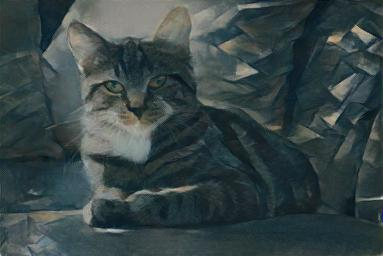
\includegraphics[width=.8\linewidth]{cat_dark1e-01jpg}
  \caption{Ratio = $10^{-2}$}
  \label{fig:sfig6}
\end{subfigure}
\caption{Content Image: Cat, Style Image: Dark}
\label{fig:fig}
\end{figure}

\noindent We can see that the implementation is not very sensitive to the relative weights used. In fact, we only see changes between Figure 10 (a) and Figure 10 (f), which makes sense as those ratios are on the extremes of what we tested.

\subsection{VGG 19 vs. VGG 16 Image Embedding Results}

The first step on our implementation is to use a pretrained image classification network to build our content and style image representations. We would like to test how sensitive our algorithm is to the choice of neural network used. The hyperparameters for this run were $iterations = 8000, \frac{Content Weight}{Style Weight} = 10^{-7}, and seed = 1$. The difference between VGG-16 and VGG-19 is that VGG-19 has three additional convolutional layers that VGG-16 does not have. [3] The results for VGG-19 vs. VGG-16 are below:

\begin{figure}[H]
\begin{subfigure}{.5\textwidth}
  \centering
  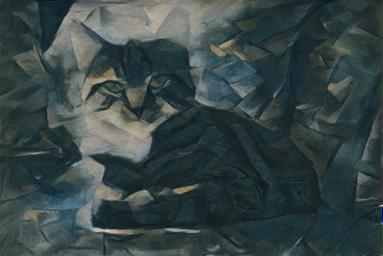
\includegraphics[width=.8\linewidth]{cat_dark19}
  \caption{VGG w/ 19 layers}
  \label{fig:sfig1}
\end{subfigure}
\begin{subfigure}{.5\textwidth}
  \centering
  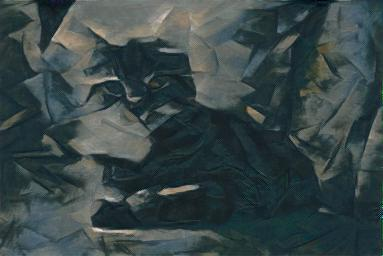
\includegraphics[width=.8\linewidth]{cat_dark16}
  \caption{VGG w/ 16 layers}
  \label{fig:sfig2}
\end{subfigure}
\caption{Content Image: Cat, Style Image: Dark}
\label{fig:fig}
\end{figure}

\noindent VGG with 19 layers is much more realistic than VGG with 16 layers. We can see this as the colors in VGG-16 are dark to the point of almost compromising the cat's structure. It makes sense to use VGG with 19 layers for image blending applications especially when deploying in cloud environments with less demanding memory constraints.

\subsection{Loss over Training Iterations}

If our algorithm is working we expect the loss to decrease as the number of training iterations increases. The hyperparameters for this run were $iterations = 8000, \frac{Content Weight}{Style Weight} = 10^{-7}, seed = 1$, and the image embeddings used are from VGG with $19$ layers. The results for our cat content image and dark style image are below:

\begin{figure}[H]
    \centering
    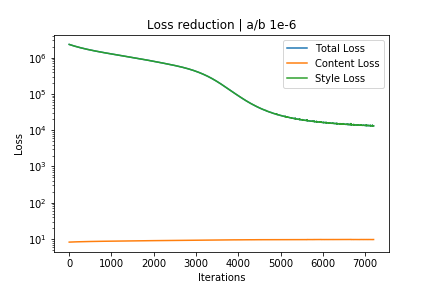
\includegraphics[height=5cm,width=10cm]{Loss}
    \caption{Loss vs. Iteration Number}
    \label{fig:sfig1}
\end{figure}

Note that the Style Loss line is practically overlaid on top of the Total Loss line, indicating that the decrease in Total Loss is due to the Style Loss decreasing. The Content Loss is a very small percentage of the Total Loss. This makes sense as we weigh our Style Loss more heavily in the calculation of the Total Loss.

\subsection{Performance over CPU vs. GPU}

The speed of CNNs is highly dependent on the hardware it is being run on. We can implement our project on GPUs on Google Colab hardware. Underneath the hood, all that is being done is matrix operations that can be parallelized. [4] The hyperparameters for this run were $iterations = 8000, \frac{Content Weight}{Style Weight} = 10^{-7}, seed = 1$, and the image embeddings used are from VGG with $19$ layers. The timing result for the cat content image and dark style image is below:

\begin{figure}[H]
    \centering
    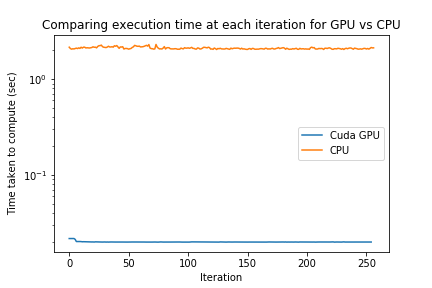
\includegraphics[height=5cm,width=10cm]{GPU_CPU_time_comparision}
    \caption{Timing, CPU vs. GPU}
    \label{fig:cpugpu}
\end{figure}

Performance on the GPU was $200x$ faster than the performance on the CPU. Also note that the time for each iteration is constant for both GPUs and CPUs. If you have the ability to transfer your computing to GPUs you should, as the speedup is massive.

\subsection{MAST Algorithm Results}

Our extension, Multi-Artist Style Transfer, or MAST, tries to incorporate $k$ style images for $1$ content image. Here we show results for $k = 2$ with the cat content image, the Starry Night as the first style image, and a minimalist image as our second style image:

\begin{figure}[H]
    \centering
    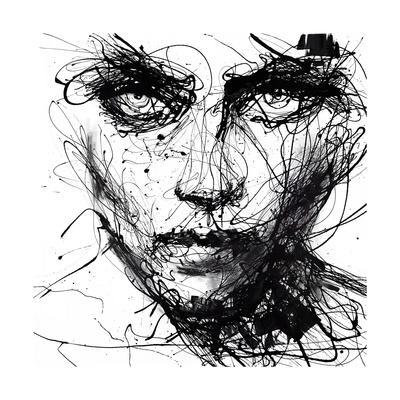
\includegraphics[height=5cm,width=5cm]{minimalistPrint}
    \caption{Second Style Image: Minimalist Drawing}
    \label{fig:cpugpu}
\end{figure}

We tried different relative weights for the two style images to show what the blended image looks like for different configurations. The hyperparameters for this run were $iterations = 8000, \frac{Content Weight}{Style Weight} = 10^{-7}, seed = 1$, and the image embeddings used are from VGG with $19$ layers. The results are below:

\begin{figure}[H]
\begin{subfigure}{.5\textwidth}
  \centering
  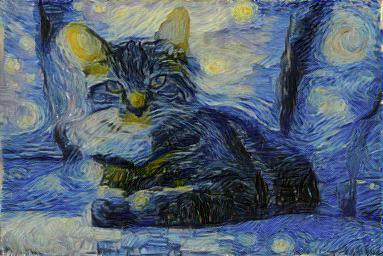
\includegraphics[width=.8\linewidth]{i0}
  \caption{Relative Weights, Style Image 1: 1, Style Image 2: 0}
  \label{fig:sfig1}
\end{subfigure}
\begin{subfigure}{.5\textwidth}
  \centering
  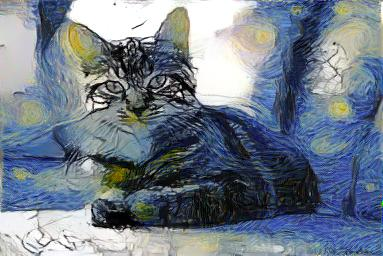
\includegraphics[width=.8\linewidth]{i25}
  \caption{Relative Weights, Style Image 1: 0.75, Style Image 2: 0.25}
  \label{fig:sfig2}
\end{subfigure}
\begin{subfigure}{.5\textwidth}
  \centering
  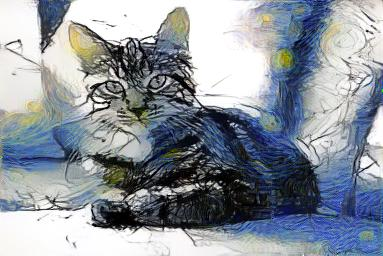
\includegraphics[width=.8\linewidth]{i50}
  \caption{Relative Weights, Style Image 1: 0.5, Style Image 2: 0.5}
  \label{fig:sfig3}
\end{subfigure}
\begin{subfigure}{.5\textwidth}
  \centering
  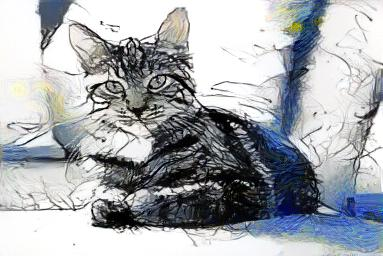
\includegraphics[width=.8\linewidth]{i75}
  \caption{Relative Weights, Style Image 1: 0.25, Style Image 2: 0.75}
  \label{fig:sfig4}
\end{subfigure}
\begin{subfigure}{.5\textwidth}
  \centering
  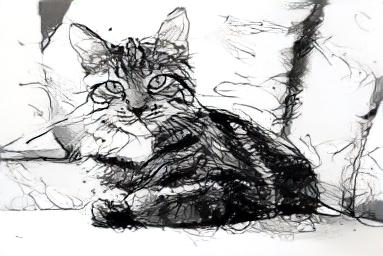
\includegraphics[width=.8\linewidth]{i1}
  \caption{Relative Weights, Style Image 1: 0, Style Image 2: 1}
  \label{fig:sfig5}
\end{subfigure}
\caption{Content Image: Cat, Style Image 1: Starry Night, Style Image 2: Minimalist Drawing}
\label{fig:fig}
\end{figure}

We can see that the MAST algorithm works as expected, the cat image is being created as if two different artists were painting it. We can also see that as the relative weight of the two style images varies the content image moves in that direction.

\section{Conclusion}

We use the Neural Algorithm of Artistic Style with VGG to build content and style representations. Then we run gradient descent over the output image, optimizing for total loss - a weighted sum of the content and style loss. After being satisfied with the accuracy of the algorithm's implementation, we tested its robustness to various factors like the number of training iterations, the initial random seed, and the relative weights of the content and style loss in the total loss function. Due to the amount of time it takes to run the algorithm we had to implement a version that used GPU operations. This provided us with close to a 200x speedup. We show how effective the algorithm is in producing realistic images over a variety of content and style combinations. Lastly, we proposed a new extension of Neural Algorithm of Artistic Style for Many-Artist Style Transfer (MAST) where the total style loss at each iteration is a weighted sum of the style loss over each style image. The results show a remarkable ability for the CNN to blend multiple style images together onto one content image. In the future, we hope to develop methodology to combine multiple non-overlapping sets of content and style images into k output images.

\section*{References}

[1] Simonyan, Karen \& Zisserman, Andrew. (2014). Very Deep Convolutional Networks for Large-Scale Image Recognition. arXiv 1409.1556.

\noindent [2] L. Gatys, A. Ecker, and M. Bethge, ‘‘Image style transfer using convolutional neural networks,’’ in Proc. IEEE Conf. Comput. Vis. Pattern Recognit. (CVPR), Jun. 2016, pp. 2414–2423.

\noindent [3] Rosebrock, Adrian. “ImageNet: VGGNet, ResNet, Inception, and Xception with Keras.” PyImageSearch, 5 Feb. 2019, www.pyimagesearch.com/2017/03/20/imagenet-vggnet-resnet-inception-xception-keras/.

\noindent [4] Baltazar, Gino. “CPU vs GPU in Machine Learning.” Oracle Data Science, blogs.oracle.com/datascience/cpu-vs-gpu-in-machine-learning.

\end{document}